


\documentclass[12pt, letterpaper]{article}

\usepackage[T1]{fontenc} 		%Font choice
\usepackage[margin=1in]{geometry}
\usepackage{graphicx}
\usepackage{amssymb}
\usepackage{mathtools}
\usepackage[chaptertitle=true,articletitle=true,biblabel=period]{achemso} 		%Use Achemso package etalmode=firstonly,maxauthors=3,
\usepackage{fancyheadings}
\usepackage{color}
\usepackage{float}
%\floatstyle{boxed}
\restylefloat{figure}
\usepackage{gensymb}
\usepackage{booktabs} % Allows the use of \toprule, \midrule and \bottomrule in tables for horizontal lines

\usepackage{caption}
\usepackage{subcaption}

\usepackage{fixltx2e} %subscripts...

\usepackage[font=small,labelfont=bf]{caption}


\title{Liquid Argon - Molecular Dynamics simulation in NVE and NPT; Analysis update}
\author{Russell Davidson}

\begin{document}\thispagestyle{empty}
\maketitle

\paragraph{Mean-squared Displacement Analysis.}
The mean-squared displacement (MSD) of the argon atoms within the 512-atom liquid argon system was calculated for a NVE, homebrew MD simulation. For this simulation, the coordinates and velocities were written every 10 steps, with a time step of 2 fs. The MSD values were calculated by measuring the distance moved by each atom over time. Figure \ref{fig:msd} shows the MSD graph for the NVE simulation of liquid Argon at ~230 K. 

\begin{figure} [p]
	\centering
	\caption{ Mean-squared displacement versus time for the NVE liquid Argon simulation. The slope of the linear region of this plot is equal to 6D, where D is the self-diffusion coefficient of liquid argon. For this graph, D equals 5.495E-09 $m^{2}\ s^{-1}$.} 
	\frame{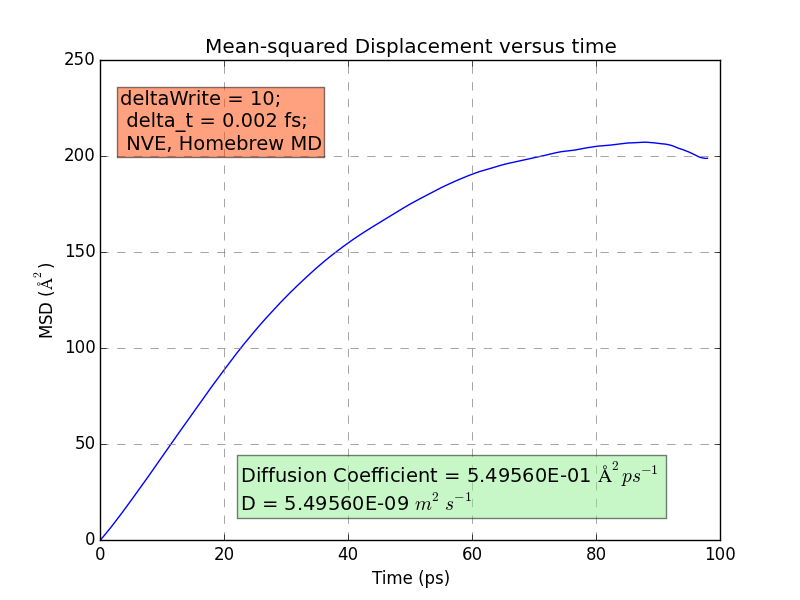
\includegraphics[width=\textwidth] {../Analysis/MSD/MSD.png}}
	\label{fig:msd}
\end{figure}

\paragraph{Velocity Autocorrelation Analysis.}
The velocity autocorrelation (VAC) of the argon atoms in the simulation described above was calculated using the Green-Kubo algorithm. Figure \ref{fig:vac} shows the VAC graph for liquid Argon at ~230K.

\begin{figure} [p]
	\centering
	\caption{Velocity Autocorrelation versus time for the NVE liquid Argon simulation. The integral of the VAC for all times corresponds to the self-diffusion coefficient, D. For this simulation, D equals 2.487E-05 $m^{2}\ s^{-1}$.}
	\frame{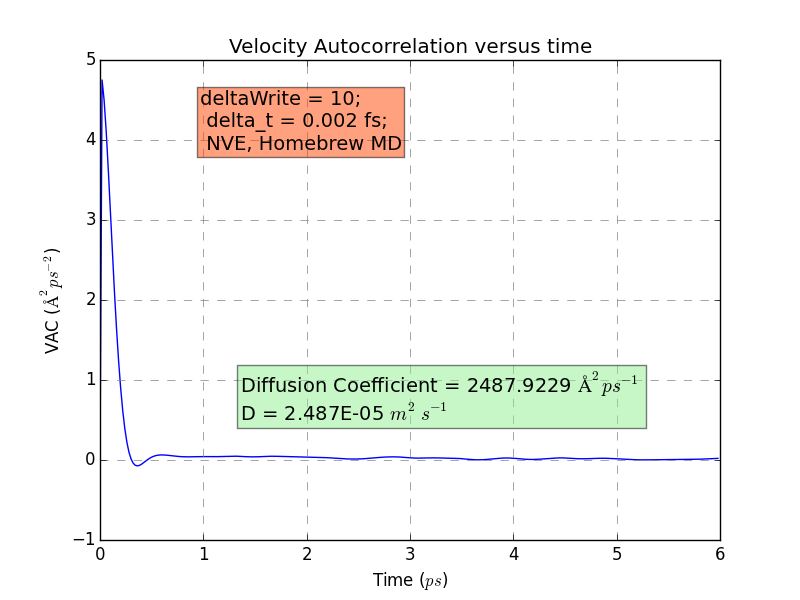
\includegraphics[width=\textwidth] {../Analysis/VAC/VAC.png}}
	\label{fig:vac}
\end{figure}

The self-diffusion coefficients calculated from MSD and VAC analysis methods do not correlate very well. It is possible that a deltaWrite value of 10 steps is still too many steps between writing coordinates and velocities. This would be especially deleterious to the VAC method since the correlation and anti-correlation of velocities should occur very quickly. With a 10 step value, the current VAC analysis does not observe correlation or anti-correlation behavior that occur on shorter timescales (< 20 fs). This smoothing over of the VAC might explain why the diffusion coefficient is much larger for the VAC than the MSD anlaysis, since the running integral is dependent on observing correlated and anti-correlated states. 

\paragraph{Radial Distribution Function.}
For the same simulation as described above, the radial distribution function (RDF) of the Argon atoms was calculated. Figure \ref{fig:rdf} shows the RDF graph for the liquid argon simulation. 

\begin{figure} [p]
	\centering
	\caption{Radial distribution versus distance for the NVE liquid Argon simulation. For this simulation, the system was condensed enough to observe two solvation shells, occurring (approximately) at 3.5 and 6.5 \AA\ .}
	\frame{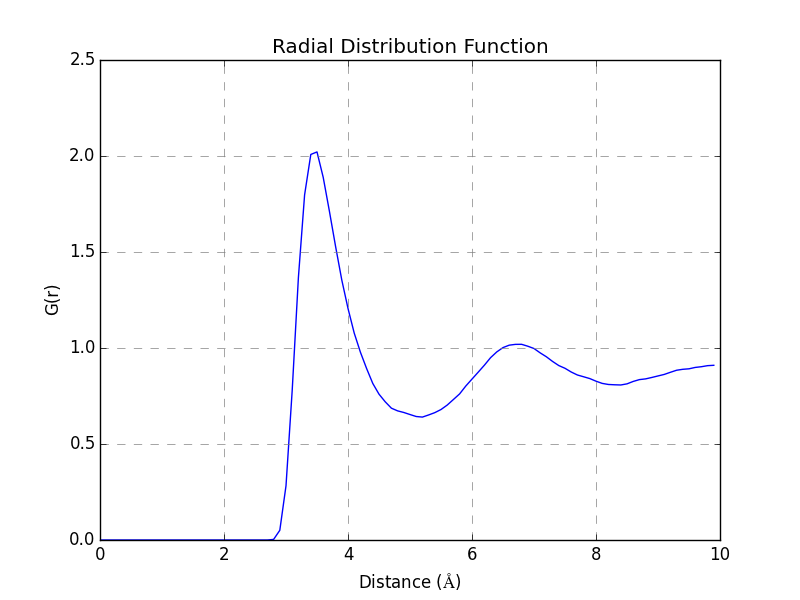
\includegraphics[width=\textwidth] {../Analysis/RDF/RDF.png}}
	\label{fig:rdf}
\end{figure}

\paragraph{Potential of Mean Force.}
Using the reversible work theorem, the potential of mean force (PMF) of moving two argon atoms from infinite distance away to short distances was calculated from the RDF discussed above. Simply, the PMF was calculated by taking the -log of the RDF and multiply by RT. Figure \ref{fig:pmf} shows the PMF graph for moving two Argon atoms from large distances to short distances. 

\begin{figure} [p]
	\centering
	\caption{Potential of mean force versus distance for two Argon atoms, as simulated from the NVE liquid Argon simulation. Sampling of distances shorter than 2.8 \AA\ was insufficient due to the high repulsive Lennard-Jones forces present at such distances. The PMF at these short distances are not shown but were calculated to be infinity. Enhanced sampling methods should be used to obtain more complete PMF graphs.}
	\frame{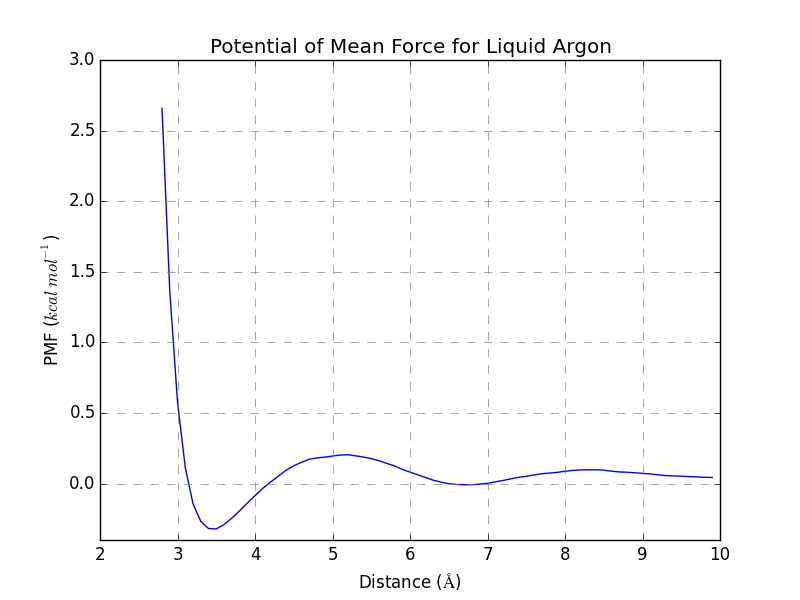
\includegraphics[width=\textwidth] {../Analysis/RDF/PMF.png}}
	\label{fig:pmf}
\end{figure}





\end{document}






